\documentclass[a4paper,oneside,article,11pt]{memoir}
\usepackage[english]{babel}
\usepackage[utf8]{inputenc}
\usepackage{amsmath,amssymb,amsthm}

% This font looks so good.
\usepackage[sc]{mathpazo}

% Typesetting pseudo-code
\usepackage{algorithm}
\usepackage{algorithmic}
\usepackage{multirow}
% Code comments like [CLRS]
\renewcommand{\algorithmiccomment}[1]{\makebox[5cm][l]{$\triangleright$ \textit{#1}}}
\usepackage{framed,graphicx,xcolor}
\usepackage[font={small,it}]{caption}
\usepackage{listings}
\usepackage{units}

% Relative references
\usepackage{varioref}

\usepackage{hyperref}

\bibliographystyle{plain}

\title{Advanced Data Structures \\ Project 2 - van Emde Boas Trees}
\author{Peter Gabrielsen 20114179 \\
Christoffer Hansen 20114637}
\newcounter{qcounter}
\begin{document}

\begin{titlingpage}
\clearpage

\maketitle
\thispagestyle{empty}

\begin{abstract}
This project aims to compare the practical performance of \textit{van Emde Boas Trees} with \textit{Red-Black Trees} and priority queues using \textit{Fibonacci}, \textit{Binary} heaps respectively. We will conduct experiments that tests the experimental performance of each of the basic priority queue operations: \texttt{Insert}, \texttt{DeleteMin}, \texttt{FindMin}, and \texttt{DecreaseKey} on the heaps and the \textit{van Emde Boas Tree}. Furthermore we will test the operations: 
\texttt{MakeQueue}, \texttt{Delete} and \texttt{PredecessorSearch} on the \textit{Red-Black Tree} and \textit{van Emde Boas Tree}.
The experiments will test the data structures in the average and in the worst case situation.

The results of all the operations align very good with the theoretical bounds in the worst case.

We record an overall tendency of better running times on the \textit{Fibonacci}, \textit{Binary} heaps and \textit{Red-Black} trees compared against \textit{van Emde Boas} trees on all practical values of $n$ except for the operations \texttt{Delete} and \texttt{PredecessorSearch} where we find the \textit{van Emde Boas tree} to outperform the \textit{Red-Black tree}. %TODO explain why the constant is big in the \log \log u aysomtotic bound on the van Emde Boas tree.
\\
\\
\\
The code can be found at: \\\url{https://dl.dropboxusercontent.com/u/8990890/2015Q1Q2_ADS_20114179_20114637_Project2.zip}.
\end{abstract}
\end{titlingpage}

\pagebreak

\tableofcontents

\pagebreak

\chapter{Introduction}
van Emde Boas trees are interesting since they circumvent the sorting bound by restricting the keys in the data structure to be from $0$ to $n-1$ and with no duplicates similar to counting sort. With this restriction it allows the priority queue operations and some more in $\mathcal{O}(\log\log n)$ worst case time. In this project we will let our universe be 24-bit integer keys. We will run experiments that compare the van Emde Boas tree's priority queue operations to the binary heap~\cite{williams} and the Fibonacci heap~\cite{fred87}. Our findings can be found in section~\ref{chap:pqe}.

The van Emde Boas tree also supports finding the predecessor of an element in $\mathcal{O}(\log\log u)$ time which we will experimentally compare to the $\mathcal{O}(\log n)$ time of the Red-Black tree. We will also experimentally compare other tree operations for these two trees. The results of these experiment are found in section~\ref{chap:treee}
\chapter{Implementation}
\label{cpt:implementation}


\subsection{van Emde Boas tree}
The van Emde Boas tree was implemented as described in Introduction to Algorithms~\cite{clrs}. It is a non space-reduced tree and as such it will take time proportional to allocating the full universe of the tree in memory, to construct such a tree. However the tree will not grow in memory after allocation. A way to mitigate this, and thereby make the tree space-reduced would be to, instead of storing the complete structure, we should only store the substructures that actually contain elements. This could have been implemented by using hash maps instead of arrays.

Decrease key in the van Emde Boas tree was implemented as a delete and an insert giving an $\mathcal{O}(\log\log u)$ bound for this operation. The other asymptotic bounds for the van Emde Boas tree can be found in table~\ref{tab:van_emde_boas}.
\begin{figure}[H]
\begin{center}
\begin{tabular}{c|c}
Operation & Running time \\\hline
\texttt{FindMin} & $\mathcal{O}(1)$ \\\hline
\texttt{Insert} & $\mathcal{O}(\log\log u)$ \\\hline
\texttt{Delete} & $\mathcal{O}(\log\log u)$ \\\hline
\texttt{DeleteMin} & $\mathcal{O}(\log\log u)$ \\\hline
\texttt{PredecessorSearch} & $\mathcal{O}(\log\log u)$ \\\hline
\texttt{DecreaseKey} & $\mathcal{O}(\log\log u)$
\end{tabular}
\end{center}
\caption{Asymptotic running time for the van Emde Boas tree}
\label{tab:van_emde_boas}
\end{figure}

%TODO no page faults since we load everything in memory at beginning!

\subsection{Red-Black tree}
The Red-Black tree was implemented as described in Introduction to Algorithms~\cite{clrs}.

The Red-Black tree is a very popular balanced binary search tree and supports basic dynamic-set operations in time $\mathcal{O}(\log n)$.

\chapter{Experimental setup}
\label{chtp:experiment_setup}
%TODO write something about the machine which ran the experiments and something about how we measure the different things. Maybe copy all this from the AE report?

The experiments were performed on a machine with a Intel i5-3210M @ 2.5GHz (Ivy Bridge) with 128K bytes of L1 cache, 512K bytes of L2 and 3072K bytes of L3 cache. The machine had 4.2GB ram and ran Ubuntu 14.04 with kernel version 3.16.0-50.

The running time was measured using the built in \texttt{high\_resolution\_clock} in the \texttt{chrono} library. This measures the wall clock. It is the clock in \texttt{c++} with the highest precision, i.e. the shortest tick period.

The code is compiled with \texttt{g++ 4.8.4} with the \texttt{c++11} standard enabled and no optimization level.

The elements in our data structures were 32 bit integers. Random elements were generated uniformly in the 32 bit integer range using the Mersenne Twister 19937 from the \texttt{random} library.

CPU measurements were collected using \texttt{PAPI 5.3.0.0}

We used \texttt{perf} to measure page faults.

\chapter{Priority queue experiments}
\label{chap:pqe}
In this section we will design and perform experiments where we compare the van Emde Boas tree based priority queue with more standard priority queue implementations, namely the Fibonacci heap and binary heap. We will for each priority queue operation describe the experiments, present the results of said experiments and discuss those in detail.

\section{\texttt{FindMin}}
Finding the minimum in all three priority queues are constant time operations. They all just involve returning a stored element or dereferencing a pointer. We therefore expect to see all three queues perform similar and constant in the size of the input. In this experiment we do not measure running time since this is a constant time operation. Instead we measure the number of cycles and branch operations performed when calling find minimum in the respective queues. The experiments are repeated 10 times and averaged. The results are depicted in figure~\ref{fig:findmin_br} and~\ref{fig:findmin_cyc}.

\begin{figure}[H]
\centering
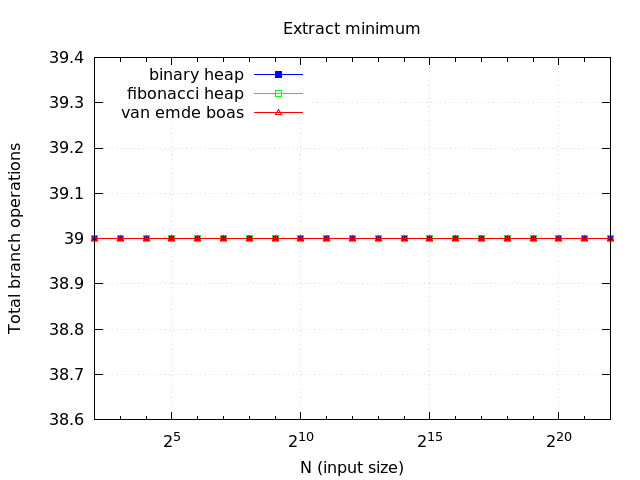
\includegraphics[scale=0.5]{../res2/findmin/extract_min_branch.png}
\caption{Number of branch operations for finding the minimum element}
\label{fig:findmin_br}
\end{figure}

\begin{figure}[H]
\centering
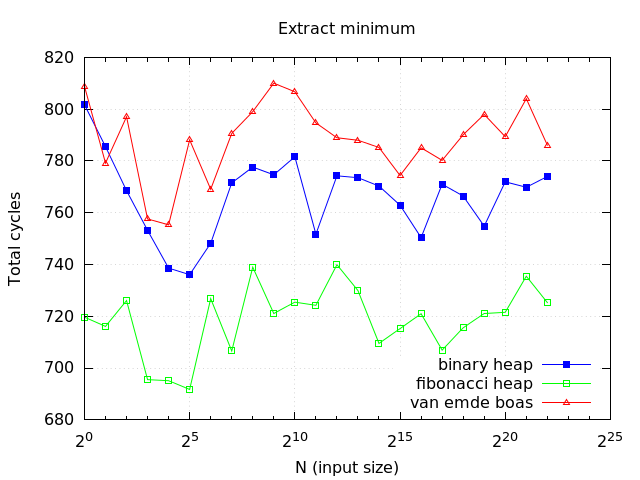
\includegraphics[scale=0.5]{../res2/findmin/extract_min_cycles.png}
\caption{Number of cycles for finding the minimum element}
\label{fig:findmin_cyc}
\end{figure}

The results clearly depict that finding the minimum does not depend on the input size and we conclude that the theoretical bound of $\mathcal{O}(1)$ also matches the experimental found results.

\section{\texttt{Insert}}
The asymptotic running times of the priority queues are as depicted in figure~\ref{fig:asymptotic_insert}.

\begin{figure}[H]
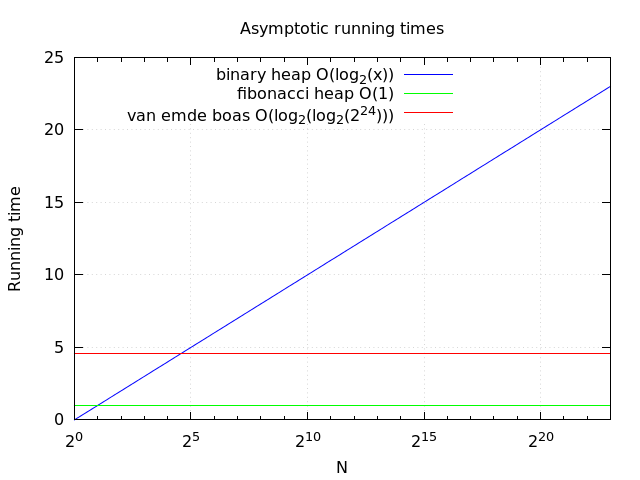
\includegraphics[scale=0.5]{../res2/inserts/runtime_plot.png}
\caption{Asymptotic running times for inserting in the priority queues.}
\label{fig:asymptotic_insert}
\end{figure}

We notice that inserting into the van Emde Boas tree does not depend on the size of the input but rather on the size of the universe that the tree hold. Since we support a universe of integers in the range from $0$ to $2^{24}$ we should have an insert that takes $\log\log 2^{24} = 4,5$ i.e. a larger constant than the Fibonacci heap but none the least a constant. What we expect to see in the worst case experiment is that the Fibonacci always performs best and at some point the van Emde Boas tree will outperform the Binary Heap with logarithmic asymptotic running time.

In order to see this result we remember from our previous experiments with priority queues that we need to experiment with the worst case data for the binary heap in order to see the logarithmic behaviour of the heap. This observation also makes it obvious that we do not want to see the behaviour of the heaps on random data since these would be similar to previous results from our first report. In figure~\ref{fig:insert_worst_running} we depict the results of running on the worst case data 10 times and averaging the result. The results confirm our hypothesis and that the running time of the van Emde Boas tree is independent of the input size while the binary heap is logarithmically dependent.

\begin{figure}[H]
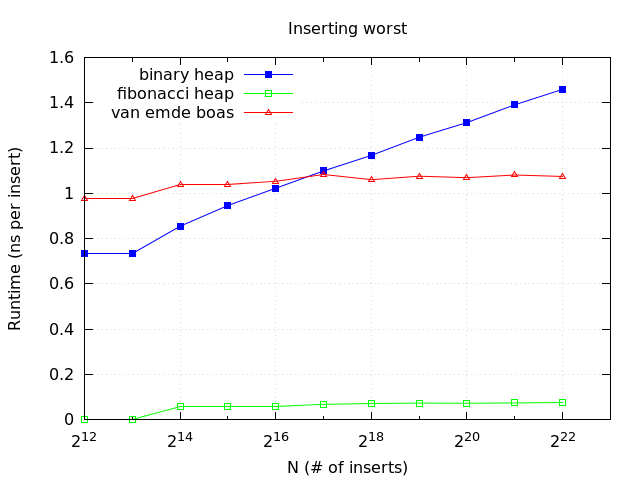
\includegraphics[scale=0.5]{../res2/inserts/runtime_worst.png}
\caption{Worst case running time for the priority queues.}
\label{fig:insert_worst_running}
\end{figure}

Looking at the number of branch operations in figure~\ref{fig:insert_worst_branch} we see that the number of branch operations is constant for the van Emde Boas tree and the Fibonacci heap while the binary heap increases logarithmically.

\begin{figure}[H]
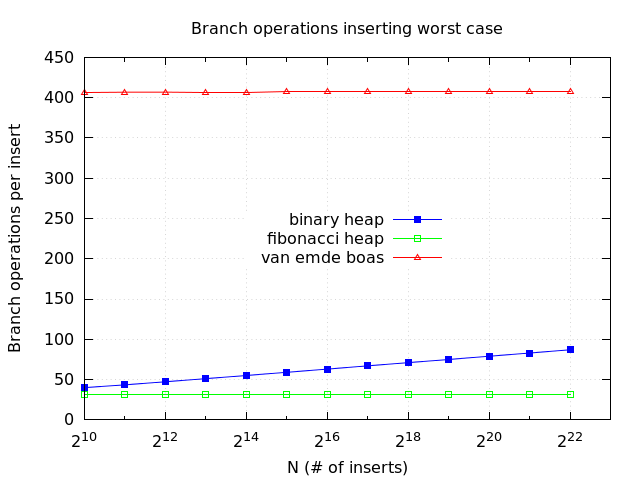
\includegraphics[scale=0.5]{../res2/inserts/branch_worst.png}
\caption{Worst case branching operations for the priority queues when inserting.}
\label{fig:insert_worst_branch}
\end{figure}


\section{\texttt{DeleteMin}}
Deleting the minimum element from a priority queue takes amortized logarithmic time for the Fibonacci heap. In the worst case it takes linear time if it is done after $n$ inserts due to the linear running time of consolidating the heap. The binary heap takes logarithmic time in the worst case since it might have to bubble the element all the way to the bottom again. The van Emde Boas tree deletes the minimum in $\mathcal{O}(\log\log u)$. In order to show these bounds experimentally we will make sure that the Fibonacci heap has consolidated and the binary heap operates in the worst case. The experiment will make two deletes to each priority queue and only measure the second. This way the Fibonacci queue has consolidated and we will only measure the amortized cost. The experiment was repeated 10 times and averaged. Since the operation is hard to measure using wall clock we measured the number of branching operations. The result of the experiment is depicted in figure~\ref{fig:insert_worst_branch}.

\begin{figure}[H]
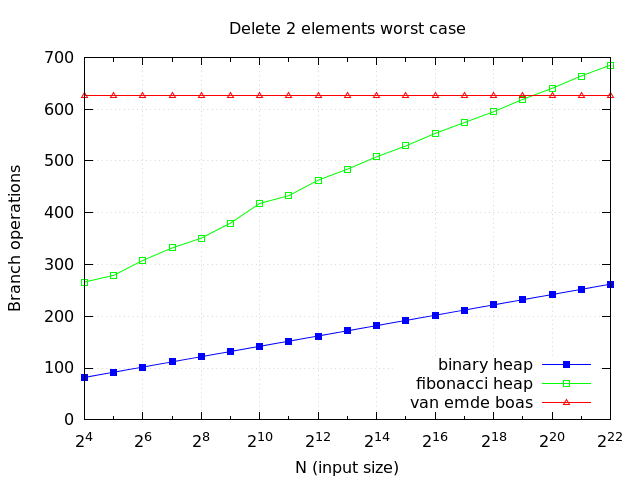
\includegraphics[scale=0.5]{../res2/delmin/delmin_del_2_branch_worst.png}
\caption{Worst case branching operations for the priority queues on delete minimum.}
\label{fig:insert_worst_branch}
\end{figure}

Figure~\ref{fig:insert_worst_branch} shows that both the binary heap and the Fibonacci heap are logarithmic in the input size while van Emde Boas remains constant in the input size as hypothesized.

\section{\texttt{DecreaseKey}}
Decreasing the key in the Fibonacci heap is an amortized constant time operation. The binary heap is logarithmic in the worst case and finally the van Emde Boas tree is as usual $\mathcal{O}(\log\log u)$. We implemented decrease key as an erase and an insert in the van Emde Boas tree.

The experiment tests the interesting worst case behaviour where we in the binary heap decrease the maximum element such that it has to bubble all the way to the top every time. The experiment first consolidates the Fibonacci heap and then runs 1 decrease key operation for various input sizes. The result are depicted in figure~\ref{fig:dk_worst_1}.

\begin{figure}[H]
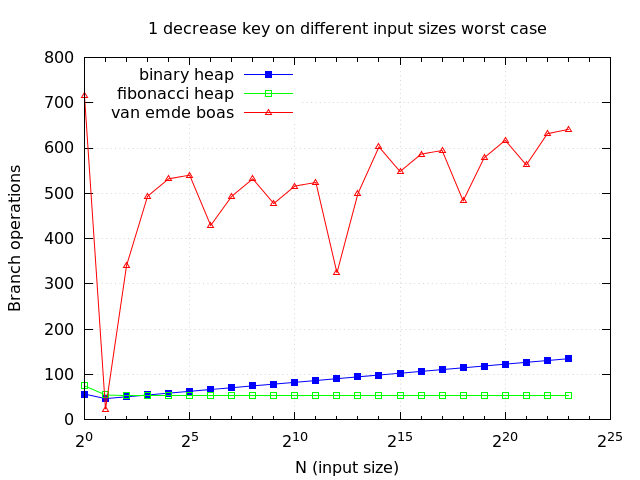
\includegraphics[scale=0.5]{../res2/dk/dk_worst_1.png}
\caption{Worst case branching operations for the priority queues on decrease key.}
\label{fig:dk_worst_1}
\end{figure}


\section{Conclusion}
Finding the minimum element took constant time for all three priority queue implementation as expected.

Insert was found to be a constant time operation for the Fibonacci heap, a $\mathcal{O}(\log\log u)$ time operation for the van Emde Boas tree, and finally a logarithmic time operation for the binary heap in the worst case.

Deleting the minimum element was found to be a constant time operation for the van Emde Boas tree, while is a logarithmic time operation for the binary heap and Fibonacci heap.

Finally decrease key was found to be constant for the Fibonacci heap, logarithmic for the binary heap and %TODO what about van emde boas

\chapter{Red-Black tree \& van Emde Boas}
\label{chap:treee}

In this section we will design and perform experiments where we compare the operations \texttt{MakeQueue}, \texttt{FindMin}, \texttt{Insert}, \texttt{DeleteMin}, \texttt{Delete} and \texttt{PredecessorSearch} on the van Emde Boas tree against our Red-Black tree implementation. For each operation we will motivate the experimental setup, present the result of said experiments and discuss those in detail.

\section{\texttt{MakeQueue}}
As we decided to implement the van Emde Boas tree in the form of a non-space reduced tree we expect that the construction will take time proportional to the size of the universe. Therefore, we conduct an experiment where we measure the construction of each of the data structures in sizes from $u \in [2^0, \dots, 2^{24}]$. We expect to see the Red-Black tree to be constructed in $\mathcal{O}(1)$ and the van Emde Boas tree to be constructed in $\mathcal{O}(u)$ time. The experiments are repeated 10 times and averaged. The results are depicted in figures~\ref{fig:rbveb_mq_pow2_rt} and~\ref{fig:rbveb_mq_pow2_logscale_y_rt}. We are pleased to see a $\mathcal{O}(1)$ construction time of the Red-Black tree in figure~\ref{fig:rbveb_mq_pow2_rt} and to see a linear growth on the van Emde Boas tree on the log-log scaled plot presented in figure~\ref{fig:rbveb_mq_pow2_logscale_y_rt}.

\begin{figure}[H]
\centering
\begin{minipage}{0.48\columnwidth}
  \centering
  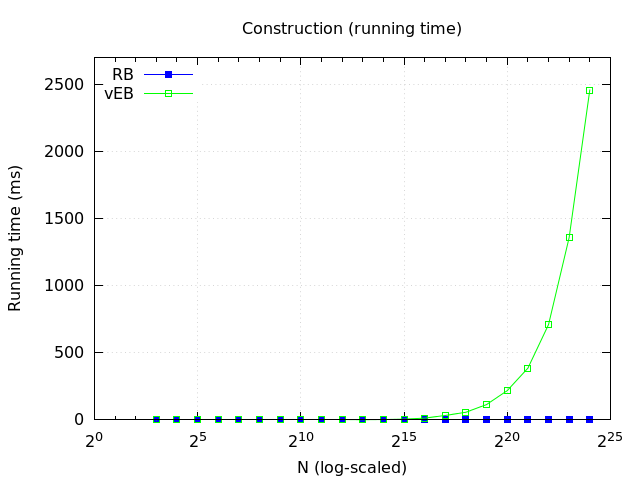
\includegraphics[width=\linewidth]{../res/rbveb/rbveb_mq_pow2_rt.png}%
  \caption{Running time for construction of Red-Black and van Emde Boas tree. X-axis is log scaled.}
  \label{fig:rbveb_mq_pow2_rt}
\end{minipage}%
\hfill
\begin{minipage}{0.48\columnwidth}
  \centering
  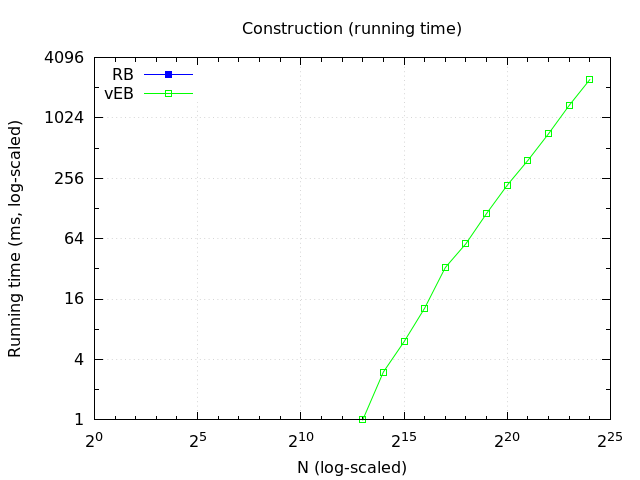
\includegraphics[width=\linewidth]{../res/rbveb/rbveb_mq_pow2_logscale_y_rt.png}%
  \caption{Running time for construction of Red-Black and van Emde Boas tree. Both axis are log scaled.}
  \label{fig:rbveb_mq_pow2_logscale_y_rt}
\end{minipage}
\end{figure}

\section{\texttt{FindMin}}

Finding the minimum in the van Emde Boas tree is a constant time operation, as we store the minimum elements outside the recursive data structure and thus can dereference a single pointer in $\mathcal{O}(1)$ time. In the Red-Black tree we have to follow the path to the left-most leaf resulting in a traversal using $\mathcal{O}(\log n)$ time. In this experiment we do not measure running time since this is a constant time operation on the van Emde Boas tree. Instead we measure the number of cycles and branch operations performed when calling find minimum in the respective queues. The experiments are repeated 10 times and averaged. The results are depicted in figure~\ref{fig:rbveb_findmin_br.png} and~\ref{fig:rbveb_mq_pow2_logscale_y_rt}.

\begin{figure}[H]
\centering
\begin{minipage}{0.48\columnwidth}
  \centering
  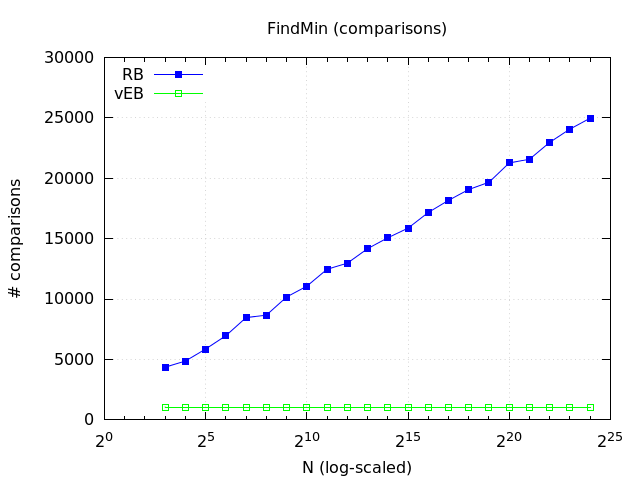
\includegraphics[width=\linewidth]{../res/rbveb/rbveb_findmin_br.png}%
  \caption{Number of branching instructions on FindMin operation on Red-Black and van Emde Boas tree.}
  \label{fig:rbveb_findmin_br.png}
\end{minipage}%
\hfill
\begin{minipage}{0.48\columnwidth}
  \centering
  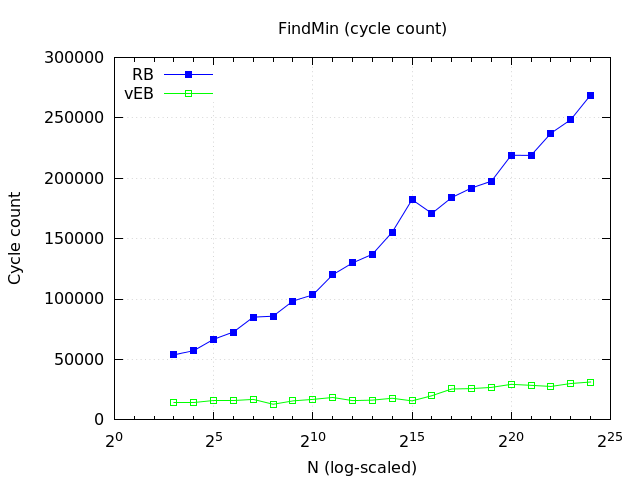
\includegraphics[width=\linewidth]{../res/rbveb/rbveb_findmin_cyc.png}%
  \caption{Total cycle count on FindMin operation on Red-Black and van Emde Boas tree.}
  \label{fig:rbveb_mq_pow2_logscale_y_rt}
\end{minipage}
\end{figure}

The results repeated in figure~\ref{fig:rbveb_mq_pow2_logscale_y_rt} clearly show that \texttt{FindMin} is a $\mathcal{O}(1)$ operation on the van Emde Boas tree and a $\mathcal{O}(\log n)$ operation on the Red-Black tree. We believe figure~\ref{fig:rbveb_findmin_br.png} shows that this can be explained by the fact that we have to find the left-most leaf in the Red-Black tree.

\section{\texttt{Insert}}
We will perform experiments on $n$ \texttt{Insert} operations on uniformly random chosen integers in the range $[0, \dots, 2^{24}-1]$ and on a sorted list of integers in the same range, as we believe the latter will make the Red-Black perform bubble each elements through all layers of the tree achieving the the worst case bound of $\mathcal{O}(\log n)$.

When inserting uniformly random distributed integers, we expect to see the running on the Red-Black tree to increase as $n$ grows, but we believe it will grow slower than the logarithmic aysmptotic analysis would suggest, as we will not bubble each element through all $\log n$ layers of the tree. We believe the van Emde Boas tree to be upper bounded by a constant.

Following the reasoning from \cite{bender}, we expect the van Emde Boas tree to be cache-oblivious. Repeating the argument we start out by looking at at the first $\nicefrac{h}{2}$ levels of the tree, where we have a subtree with $2^{\nicefrac{h}{2}}$ leaves, which again is a root of a tree of height $\nicefrac{h}{2}$.  In the van Emde Boas layout, we first lay out the rooted subtree of height $\nicefrac{h}{2}$, followed by the subtrees rooted at each leaf of this tree from left to right. Each subtree is recursively laid out using the van Emde Boas layout.

At each step of the recursion, the size of the subtrees being laid out is the square root of the size of the subtrees laid out at the previous step. Consequently, as we recurse, at some point we will be laying out subtrees with size $C$ between $\sqrt{PAGE\_SIZE}$ and $PAGE\_SIZE$. Each of these subtrees can be retrieved in a single memory transfer and this layout partitions the tree into subtrees of this size.

When finding out where to insert we access the root, which pulls in the first $\log(C)$ levels of the tree. We have only cache hits until we access a leaf of the tree, which pulls in the next $\log(C)$ levels of the tree rooted at that leaf. This continues until we reach the bottom of the tree. Because only 1 out of every $\log(C)$ accesses causes a cache miss, the total number of misses is $\nicefrac{\log n}{\log C} = \log_C n$. Since C is at least $\sqrt{PAGE\_SIZE}$ we have that $\log C$ is at least $\nicefrac{\log B}{2}$ resulting in the number of misses is at most $2 \log_B n$.

We believe the standard \textit{textbook} Red-Black tree implementation we have done builds on no cache-oblivious memory layout ideas, and so we expect the number of page faults to be low on the van Emde Boas tree relative to the Red-Black tree implementation. We are satisfied to see this hypothesis holds in the results depicted in figure~\ref{fig:rbveb_insert_pf}.

\begin{figure}[H]
\centering
\begin{minipage}{0.48\columnwidth}
  \centering
  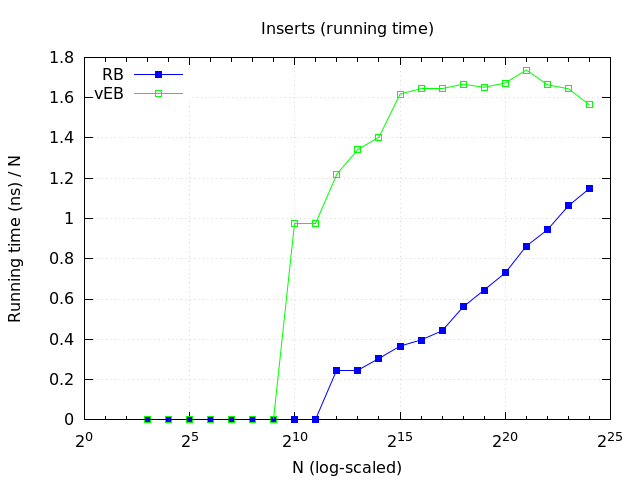
\includegraphics[width=\linewidth]{../res/rbveb/rbveb_insert_rt_div_n.png}%
  \caption{Running time per element when inserting N random uniformly random integers.}
  \label{fig:rbveb_insert_rt_div_n}
\end{minipage}%
\hfill
\begin{minipage}{0.48\columnwidth}
  \centering
  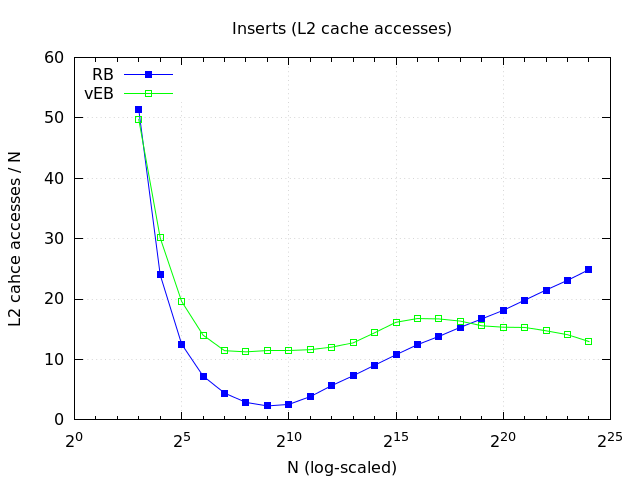
\includegraphics[width=\linewidth]{../res/rbveb/rbveb_insert_tca.png}%
  \caption{Number of L2 cache accesses per element when inserting N random uniformly random integers.}
  \label{fig:rbveb_insert_pf}
\end{minipage}
\end{figure}

In figure~\ref{fig:rbveb_insert_rt_div_n_worst_2} we present the results of inserting integers in descending sorted order. We are pleased to see that the van Emde Boas tree shows a clear tendency of being upper bounded by a constant, but we are surprised that the Red-Back tree performs better compared with inserting uniformly random integers.

\begin{figure}[H]
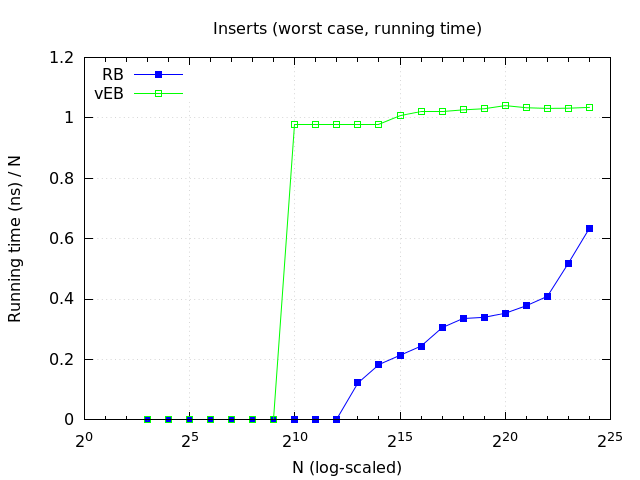
\includegraphics[scale=0.5]{../res/rbveb/rbveb_insert_rt_div_n_worst_2.png}
\caption{Inserting integers in descending sorted order.}
\label{fig:rbveb_insert_rt_div_n_worst_2}
\end{figure}

\section{\texttt{DeleteMin}}

The deletions of the minimum element is $\mathcal{O}(\log n)$ in the Red-Black tree as we have to traverse the tree to the left-most leaf which is the one we want to delete. After the deletion we have to call \texttt{erase\_fixup} that will lead to a termination after a constant amount of color changes and at most three rotations. We believe the \texttt{DeleteMin} operation is $\mathcal{O}(\log \log u)$ on the van Emde Boas tree as all we have to do is to find the second-smallest value $y$ in the vEB tree, delete it from its current location, and set it to be the minimum element. The second-smallest value $y$ is ether the maximum element or \texttt{T.children[T.aux.min].min}, and so it can be found in $\mathcal{O}(1)$ time. We conduct the experiment by performing 1000  \texttt{DeleteMin} operations on $n$ uniformly random inserted elements in the range $[0, \dots, 2^{24}-1$]. We record the total cycle count and number of branch operations required to perform the \texttt{DeleteMin} operations. The experiment was repeated 100 times and the average was used. The results are repeated in figures~\ref{fig:rbveb_deletemin_cyc} and~\ref{fig:rbveb_deletemin_br}.

\begin{figure}[H]
\centering
\begin{minipage}{0.48\columnwidth}
  \centering
  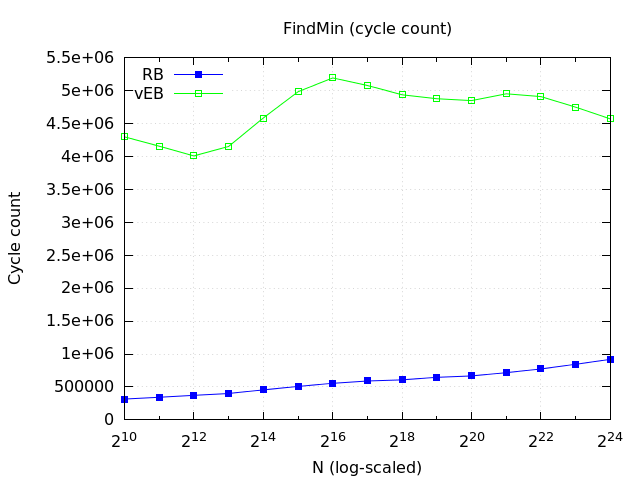
\includegraphics[width=\linewidth]{../res/rbveb/rbveb_deletemin_cyc.png}%
  \caption{Total cycle count of 1000 FindMin operations on N random uniformly random integers.}
  \label{fig:rbveb_deletemin_cyc}
\end{minipage}%
\hfill
\begin{minipage}{0.48\columnwidth}
  \centering
  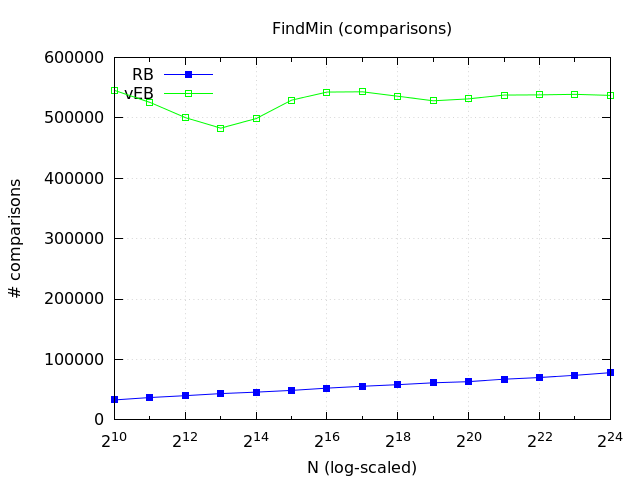
\includegraphics[width=\linewidth]{../res/rbveb/rbveb_deletemin_br.png}%
  \caption{Total number of branching operations of 1000 FindMin operations on N random uniformly random integers.}
  \label{fig:rbveb_deletemin_br}
\end{minipage}
\end{figure}

We are satisfied to see that the van Emde Boas tree is upper bounded by a constant and that the Red-Black tree measures in the order of the $\mathcal{O}(\log n)$ asympotic bound, but are surprised to the see the high number of comparisons taken to perform the 1000 \texttt{DeleteMin} operations on the van Emde Boas tree.

\section{\texttt{Delete}}
The deletions of a random element is $\mathcal{O}(\log n)$ in the Red-Black tree as we have to find the element we want to delete, which is an $\mathcal{O}(\log n)$ operation. After the deletion we have to call \texttt{erase\_fixup} that will lead to a termination after a constant amount of color changes and at most three rotations. The van Emde Boas tree deletes a random element in $\mathcal{O}(\log \log u)$. We conduct the experiment by performing 1000  \texttt{DeleteMin} operations on $n$ uniformly random inserted elements in the range $[0, \dots, 2^{24}-1$]. We record the total cycle count required to perform all of the \texttt{DeleteMin} operations. The experiment was repeated 100 times and the average was used. The result is depicted in figure~\ref{fig:rbveb_delete_cyc.png}.

\begin{figure}[H]
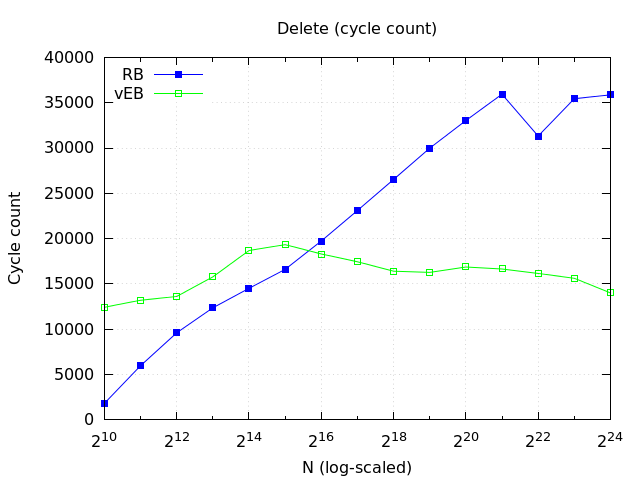
\includegraphics[scale=0.5]{../res/rbveb/rbveb_delete_cyc.png}
\caption{Total cycle count used to make 1000 Delete operations.}
\label{fig:rbveb_delete_cyc.png}
\end{figure}

We are satisfied to see that the van Emde Boas tree is upper bounded by a constant and that the Red-Black tree measures in the order of the $\mathcal{O}(\log n)$ asympotic bound, but are surprised to the see the number of comparisons taken to perform the 1000 \texttt{Delete} operations has gone dramatically down compared with the experiments done on the \texttt{DeleteMin} operation.

\section{\texttt{PredecessorSearch}}
Finding the predecessor of a inner node $x$ corresponds to finding the maximum value in its left subtree in a binary search tree. If not left child exists then the predecessor is its first left ancestor. Finding the predecessor is thus a $\mathcal{O}(\log n)$ operation on the Red-Black tree. Because we can access the maximum value in a van Emde Boas tree quickly, we can avoid making two recursive calls, and instead one recursive call on either a cluster or on the summary, but not on both. This makes the \texttt{PredSearch} operation solve to a $\mathcal{O}(\log \log u)$ operation.
We conduct the experiment by performing 1000 \texttt{Delete} operations on uniformly random integers sampled among $n$ uniformly random inserted elements in the range $[0, \dots, 2^{24}-1$]. We record the total cycle count and number of branch operations required to perform the \texttt{Delete} operations. The experiment was repeated 100 times and the average was used. The results is repeated in figure~\ref{fig:rbveb_pred_cyc}.

\begin{figure}[H]
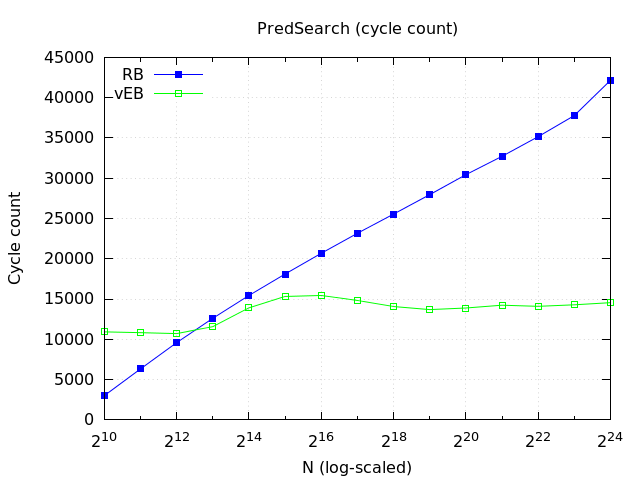
\includegraphics[scale=0.5]{../res/rbveb/rbveb_pred_cyc.png}
\caption{Total cycle count used to make 1000 PredSearch operations.}
\label{fig:rbveb_pred_cyc}
\end{figure}

\section{Conclusion}
The operations \texttt{FindMin}, \texttt{Insert}, \texttt{DeleteMin}, \texttt{Delete} and \texttt{PredecessorSearch} was found to be $\mathcal{O}(\log n)$ operations on the Red-Black tree and $\mathcal{O}(\log \log u)$ operations on the van Emde Boas tree. We found that the Red-Black tree can be constructed in $\mathcal{O}(1)$ time and that the van Emde Boas tree takes $\mathcal{O}(u)$ time using the implementation we introduced. We showed the van Emde Boas tree is cache-oblivious and provided an analysis explaining this property in terms of the memory-layout. Overall we recorded results that showed the Red-Black tree to be faster in actual running time on inserting up to $2^{24}$ elements, and severely outperforming our van Emde Boas tree on performing \texttt{DeleteMin} operations. We did however gain better running times on the van Emde Boas tree when it comes to operations \texttt{Delete} and \texttt{PredecessorSearch}.


\bibliography{references}

\end{document}


